\section{The Project}
It is believed that computers may perform better in many settings if they are able to determine the meaning of text. There are different ways of achieving these results and one of them is automatic content categorization. Automatic content categorization is a process where the text is categorized to the most describing category from a set of desirable categories. There are various ways of performing automatic content categorization. This project focus on categorizing text based on which keywords occur in the text and the keywords categories. 
%The approach for this consists of finding relevant keywords and desirable categories, create a mapping between the keywords and the categories, and then determine the most likely category for the text based the keyword occurrences. 

\begin{figure}[h]
\centering
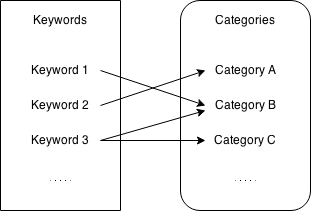
\includegraphics[width=0.65\textwidth]{Chapters/Introduction/keywordstocategories}
\caption{Illustration of the mapping between keywords and categories.}
\label{fig:keywordstocategories}
\end{figure}


Creating this automatic content categorization consists of three main steps. The first step is to create a list of keywords and a set of desirable output categories for the categorization process. For this project have we chosen titles of Wikipedia articles as keywords and the IAB taxonomy as the set of output categories. 
%The Wikipedia article titles need be processed before they can be used as keywords and some changes might be necessary to create a 
Both Wikipedia article titles and the Interactive Advertising Bureau (IAB) taxonomy might need some processing before they are suitable as keywords and a set of categories. The next step is to create a mapping between the keywords and the categories (see figure \ref{fig:keywordstocategories}. This step takes advantage of the underlying structure of Wikipedia to make sure each keyword maps to the most describing output categories. The final step of the categorization process is determine the category of any given text. This step is shown in figure \ref{fig:categorizetext} where all keywords are found in the given text and the category is determined from the keywords' categories. 

As example should an article which contains the words \emph{soccer}, \emph{Messi} and \emph{Zlatan} should probably be categorized as \emph{Sports/Soccer} if these are available keywords mapped to this category.   
%nderstanding text is important for 
%utomatic content categorization is useful for determining the meaning of a text which is useful in many settings. 
%Given a set of desirable categories it
%To be able to categorize articles, it is 
%Thus our overall goal is defined as creating a classifier that maps keywords from a predefined keyword list and to one or more pre-defined categories. The automatic categorization will include both the creation of the predefined keyword list and the mapping function, which are both essential for categorizing collections of texts based on their content. 

%Creating this automatic content categorization consists of *** steps. the first step is to find all keywords 


\begin{figure}[h]
\centering

\includegraphics[width=\textwidth]{Chapters/Introduction/categorizetext}
\caption{Simplified illustration of the categorization process.}
\label{fig:categorizetext}
\end{figure}

\begin{comment}
\begin{figure}[H]
\centering
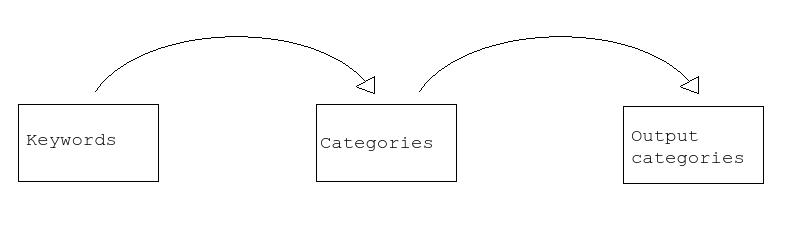
\includegraphics[width=1\textwidth]{Chapters/Introduction/classification_process.jpeg}
\caption{A simplified illustration of the categorization process.}
\label{fig:classification_process}
\end{figure}
\end{comment}
%This classifier will be used as part of an automatic categorization process. 
%Our overall goal is therefore to make an automatic categorization that have a predefined keyword list and start by creating a mapping from each keyword to a category from another predefined list. Where the category of a text can be defined from the keywords found in the text. 

\section{An Overview of Challenges}
The main challenges encountered had to do with Wikipedia, mainly because the encyclopedia is maintained by thousands of volunteers and is poorly documented from a developer's point of view. The structure of Wikipedia is complex and the size makes it hard to check if the results found are correct. 

%which also leads to a complicated and complex structure. 

\subsubsection{Encoding}
Wikipedia is available in multiple languages and is written by volunteers from all over the world. This makes Wikipedia a multilingual encyclopedia with knowledge available from everywhere and it is possible for experts form various fields and from different parts of the world to contribute with knowledge. There are both advantages and disadvantages with a multilingual encyclopedia. A disadvantage with this is that users might write with different encoding, for instance \emph{utf8}, \emph{ascii} or \emph{unicode}. Problems occur when going through all the names of Wikipedia categories and Wikipedia article titles because titles writtin in different encoding might not be viewed as identical by the computer. 

An example of a category name which leads to trouble with encoding is  \emph{Communes in Cara\cb{s}-Severin County}, which is either be written with the letter \emph{\cb{s}} \cite{swithcomma} or \c{s} \cite{swithcedilla}. These letters are examples of characters that makes matching category names difficult, because \emph{Communes in Cara\cb{s}-Severin County} and \emph{Communes in Cara\c{s}-Severin County} will not be equal to the computer even though it is clear to most users that they should be the same.

One way of solving this problem is to find

% Categorier som jeg ikke får til : 
10800


%It was not completely possible to overcome this problem, 




\subsubsection{The Structure of Wikipedia}
Another problem encountered is the underlying structure of Wikipedia which is quite complex. There are some documentations on different entries and variables in database tables, but the descriptions are short. 

Hence understanding the meaning of category names, 
Hva ligger i hvilke filer?
%The underlying structure of Wikipedia is quite complex, which led to 

\subsubsection{Creating a mapping to desirable output}


\subsubsection{Disambiguation}
A word is ambiguous if there is more than one meaning to the words. Wikipedia contains many titles with different meanings (see figure \ref{fig:disambiguation_example}), which leads to the disambiguation problem. Disambiguation is a common problem in natural language processing \cite{wiki:disambiguation}. Hence, a complete section (\ref{sec:disambiguation}) is dedicated to others solutions with this specific problem. 
%others work within in the topic see \ref{sec:disambiguation}

\begin{figure}[h]
\centering
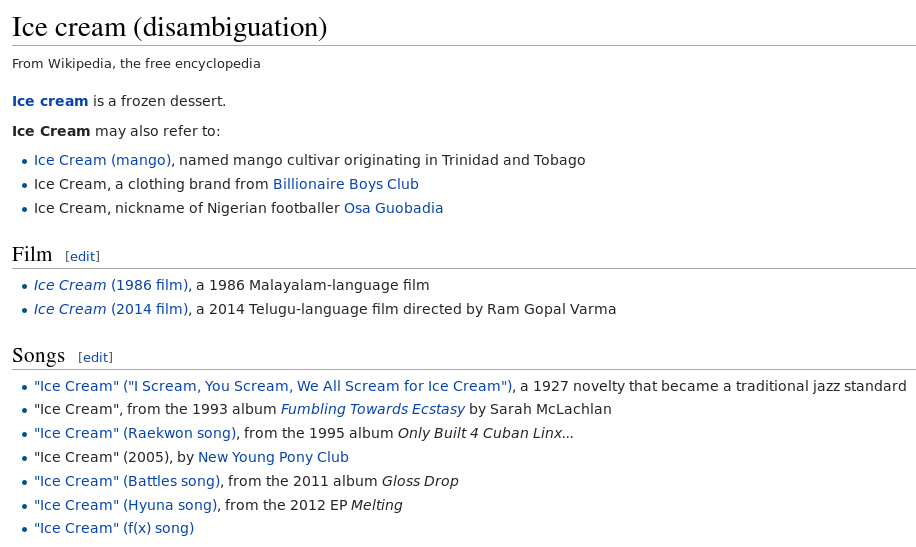
\includegraphics[width=\textwidth]{Chapters/Introduction/Ice_cream_disambiguation}
\caption{Example of disambiguation in Wikipedia.}
\label{fig:disambiguation_example}
\end{figure}